\documentclass[tikz]{standalone}

\usepackage{pgf}
\usepackage{tikz}
\usetikzlibrary{calc}
\usetikzlibrary{shadows}
\usetikzlibrary{arrows}
\usetikzlibrary{positioning}
\usetikzlibrary{shapes}
\usetikzlibrary{shadows}
\usetikzlibrary{3d}
\usetikzlibrary{arrows}
\usetikzlibrary{decorations.pathreplacing}

\begin{document}



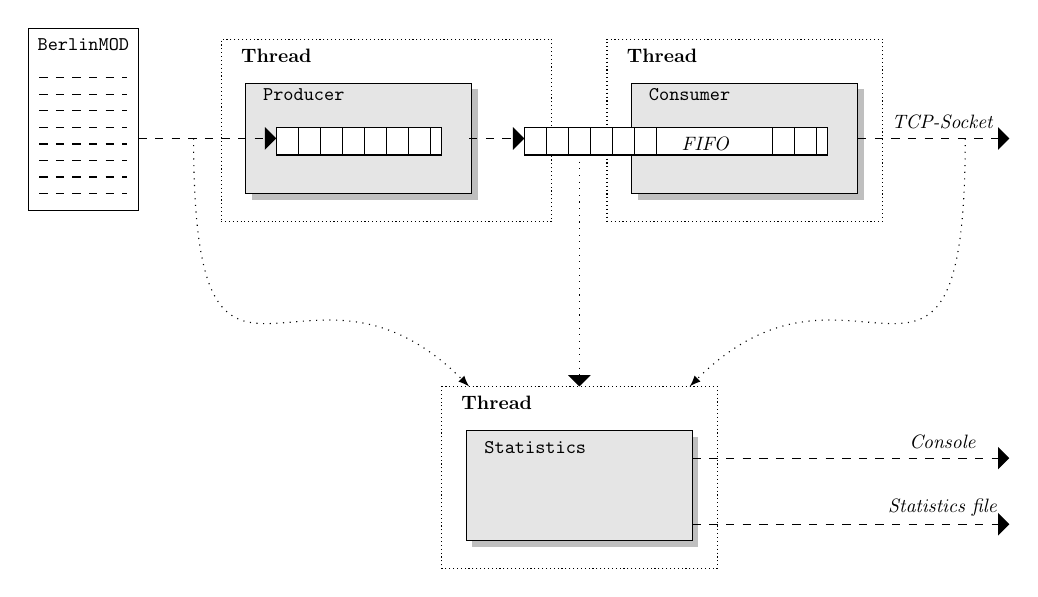
\begin{tikzpicture}[scale=0.7,  every node/.style={transform shape}]

\path[draw] (0, -0.3) -- (2, -0.3) -- (2, 3) -- (0, 3) -- cycle; 
\foreach \k in {0, 0.3, ..., 2.3} {
   \path[draw, dashed] (0.2, \k) -- (1.8, \k); 
}

\node at(1,2.7) {\texttt{BerlinMOD}};

\path[draw, densely dotted] (3.5, -0.5) -- (9.5, -0.5) -- (9.5, 2.8) -- (3.5, 2.8) -- cycle ; 
\node at(4.5,2.5) {\textbf{Thread}};

\node [draw, drop shadow, fill=gray!20, minimum width=4.1cm, minimum height=2cm] at (6,1) (out1) {}; 
\path[draw, fill=white] (4.5, 1.2) -- (7.5, 1.2) -- (7.5, 0.7) -- (4.5, 0.7) -- cycle; 
\node at(5,1.8) {\texttt{Producer}};

\foreach \k in {4.5, 4.9,...,7.5} {
   \path[draw] (\k, 1.2) -- (\k, 0.7);
}

\path[draw, densely dotted] (10.5, -0.5) -- (15.5, -0.5) -- (15.5, 2.8) -- (10.5, 2.8) -- cycle ; 
\node at(11.5,2.5) {\textbf{Thread}};

\node [draw, drop shadow, fill=gray!20, minimum width=4.1cm, minimum height=2cm] at (13,1) (out2) {}; 
\path[draw, fill=white] (9, 1.2) -- (14.5, 1.2) -- (14.5, 0.7) -- (9, 0.7) -- cycle; 
\node at(12,1.8) {\texttt{Consumer}};

\node at(12.3,0.9) {\emph{FIFO}};

\foreach \k in {9, 9.4,...,11.5} {
   \path[draw] (\k, 1.2) -- (\k, 0.7);
}

\foreach \k in {13.5, 13.9,...,14.5} {
   \path[draw] (\k, 1.2) -- (\k, 0.7);
}

\path let \p1=(out2.east) in (2, \y1) edge[-triangle 90, dashed] (4.5, \y1);
\path let \p1=(out2.east) in (8, \y1) edge[-triangle 90, dashed] (9, \y1);
\path let \p1=(out2.east) in (\x1, \y1) edge[-triangle 90, dashed] (17.8, \y1);
\node at(16.6,1.3) {\emph{TCP-Socket}};

\path[draw, densely dotted] (7.5, -3.5) -- (12.5, -3.5) -- (12.5, -6.8) -- (7.5, -6.8) -- cycle ; 
\node [draw, drop shadow, fill=gray!20, minimum width=4.1cm, minimum height=2cm] at (10,-5.3) (out0) {}; 
\node at(8.5,-3.8) {\textbf{Thread}};
\node at(9.2, -4.6) {\texttt{Statistics}};

\draw[->, >=latex, dotted] (3, 1) .. controls (3, -5) and (5, -0.5) .. (8, -3.5);
\path (10, 0.7) edge[-triangle 90, dotted] (10, -3.5);
\draw[->, >=latex, dotted] (17, 1) .. controls (17, -5) and (15, -0.5) .. (12, -3.5);

\node at(16.6,-4.5) {\emph{Console}};
\node at(16.6,-5.7) {\emph{Statistics file}};
\path let \p1=(out0.east) in (\x1, -4.8) edge[-triangle 90, dashed] (17.8, -4.8);
\path let \p1=(out0.east) in (\x1, -6) edge[-triangle 90, dashed] (17.8, -6);
\end{tikzpicture}

\end{document}
